\section{未知场与方程}
\label{sec:pdeprob-fields}

常微分方程的未知量是随时间变化的有限维向量。未知量变成空间上的函数之后，方程要写什么？这种方程和常微分方程有多少相同、从哪里开始不同？

\paragraph{从状态向量到场}
设细棒占据区间$[0,1]$。棒很细，同一截面上的温度可以看成相同，于是在时刻$t$、位置$x$处只有一个温度$u(x,t)$。固定$t$，整条曲线$x\mapsto u(x,t)$就是这一时刻棒的状态。

把棒等分为$N+1$段，步长$h=1/(N+1)$，只记录内部格点$x_j=jh$处的温度，就得到一个$N$维向量，这正是常微分方程意义下的状态。图~\ref{fig:pdeprob-state-to-field}画出同一条温度曲线在两种步长下的采样：格点加密时向量变长，竖线越来越密地铺满曲线下方。

\begin{BookInlineFigure}
  \centering
  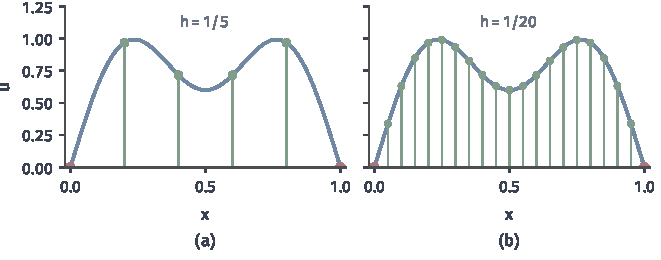
\includegraphics[width=112.0mm]{figures/06-differential-equations/02-partial-differential-equations/matplotlib/pdeprob-state-to-field/figure.pdf}
  \caption{细棒上的温度曲线（蓝）及其格点采样（绿）。曲线为$u=\sin\pi x+0.4\sin3\pi x$，两端值为零（红点）。(a)$h=1/5$，状态是$4$维向量。(b)$h=1/20$，状态是$19$维向量。把步长继续减小，向量就变成整条曲线。}
  \label{fig:pdeprob-state-to-field}
\end{BookInlineFigure}

步长趋于零时，状态不再是有限个数，而是一个函数。这样在空间每一点指定一个量的函数称为\term{场}（field）。每点的量是一个数，就是\term{标量场}（scalar field），如温度、浓度、弦的位移；每点的量是一个向量，就是\term{向量场}（vector field），如流体的速度。

\paragraph{本部分的记号}
从本章开始，空间区域记为开集$\Omega\subset\mathbb{R}^{d}$，边界为$\partial\Omega$，闭包为$\overline{\Omega}$，边界上的单位外法向为$\bm{n}$。空间点写作$\bm{x}$，一维时写作$x$。这里要特别注意：第一部分用$\bm{x}(t)$表示状态，而在这一部分$\bm{x}$只表示位置，状态的角色由整个函数$u(\cdot,t)$担任。

偏导数写作$\partial_tu$、$\partial_xu$、$\partial_{x_i}u$。三个空间微分算子只对$\bm{x}$求导，不涉及$t$，它们是：
\begin{equation}
  \begin{gathered}
    \nabla u=(\partial_{x_1}u,\ldots,\partial_{x_d}u)^{\top},\qquad
    \nabla\cdot\bm{F}=\sum_{i=1}^{d}\partial_{x_i}F_i,\\
    \Delta u=\nabla\cdot(\nabla u)=\sum_{i=1}^{d}\partial_{x_i}^{2}u.
  \end{gathered}
  \label{eq:pdeprob-operators}
\end{equation}
三者分别称为梯度、散度和Laplace算子。这些场运算的定义和计算规则与积分定理配套，可参考\BookChapterRef{chap:integral-theorems}{卷二第27章“积分定理”}。方程中其余各量的写法列在表~\ref{tab:pdeprob-notation}中，后面各章沿用。

\begin{BookInlineTable}
  \centering
  \begin{tabular}{lll}
    \toprule
    记号 & 含义 & 所在位置\\
    \midrule
    $u(\bm{x},t)$ & 未知场 & $\Omega$内 \\
    $f$ & 源项 & $\Omega$内 \\
    $u_0$ & 初值 & $t=0$的$\Omega$上 \\
    $g$ & 边值 & $\partial\Omega$上 \\
    $\bm{A}(\bm{x})$ & 扩散系数矩阵，对称正定 & $\Omega$内 \\
    $\bm{v}(\bm{x},t)$ & 速度场 & $\Omega$内 \\
    $F(u)$ & 依赖于$u$的通量 & 守恒律中 \\
    $H$ & Hamilton量 & Hamilton--Jacobi方程中 \\
    \bottomrule
  \end{tabular}
  \caption{偏微分方程部分的数据记号。}
  \label{tab:pdeprob-notation}
\end{BookInlineTable}

\paragraph{由局部守恒得到方程}
方程的形式并不是约定出来的，它来自物理量的收支。设$u$是某种量的密度，如热量或墨水浓度，$\bm{F}(\bm{x},t)$是通量，表示单位时间穿过单位面积的量，$f$是单位体积内的产生率。任取一块包含在$\Omega$内的小区域$V$，如图~\ref{fig:pdeprob-balance}。$V$内总量的变化率等于流入减去流出，再加上内部产生：
\begin{equation}
  \frac{\mathrm{d}}{\mathrm{d}t}\int_V u\,\mathrm{d}\bm{x}
  =-\int_{\partial V}\bm{F}\cdot\bm{n}\,\mathrm{d}S+\int_V f\,\mathrm{d}\bm{x}.
  \label{eq:pdeprob-balance}
\end{equation}

\begin{BookInlineFigure}
  \centering
  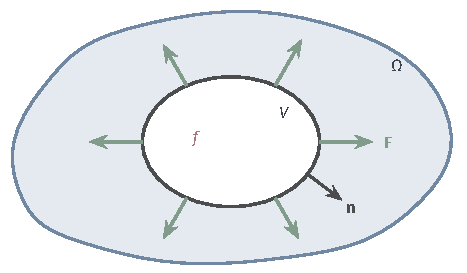
\includegraphics[width=79.1mm]{figures/06-differential-equations/02-partial-differential-equations/tikz/pdeprob-balance/figure.pdf}
  \caption{局部收支。浅蓝区域是$\Omega$，白色小区域$V$内有产生率$f$，绿色箭头表示穿过$\partial V$的通量$\bm{F}$，$\bm{n}$是$\partial V$的单位外法向。$\bm{F}\cdot\bm{n}>0$处量在流出$V$。}
  \label{fig:pdeprob-balance}
\end{BookInlineFigure}

设$u$对$t$连续可微，$\bm{F}$对$\bm{x}$连续可微，$V$的边界足够规则。由散度定理，边界积分可以改写成区域积分，式~\eqref{eq:pdeprob-balance}成为
\[
  \int_V\bigl(\partial_tu+\nabla\cdot\bm{F}-f\bigr)\,\mathrm{d}\bm{x}=0.
\]
这对每个小区域$V$都成立。被积函数连续，若它在某点为正，在该点的一个小球上也为正，取$V$为这个小球就与上式矛盾；为负时同理。所以被积函数处处为零，得到局部形式：
\begin{equation}
  \partial_tu+\nabla\cdot\bm{F}=f.
  \label{eq:pdeprob-conservation}
\end{equation}

式~\eqref{eq:pdeprob-conservation}只有一条关系，却有$u$和$\bm{F}$两个未知对象，还要说明通量怎样由$u$决定。这一步由具体的物理规律给出，不同的规律得到不同的方程。

若热量从高温流向低温，流量正比于温度梯度，就有$\bm{F}=-\bm{A}(\bm{x})\nabla u$，其中对称正定矩阵$\bm{A}$描述材料各方向的导热能力。代入后得到扩散型方程：
\begin{equation}
  \partial_tu-\nabla\cdot\bigl(\bm{A}(\bm{x})\nabla u\bigr)=f.
  \label{eq:pdeprob-diffusion-general}
\end{equation}

若量只是被流体带着走，就有$\bm{F}=\bm{v}u$。由乘积法则，
\[
  \nabla\cdot(\bm{v}u)=\bm{v}\cdot\nabla u+u\,\nabla\cdot\bm{v}.
\]
在不可压缩流动$\nabla\cdot\bm{v}=0$中，第二项消失，方程成为输运形式$\partial_tu+\bm{v}\cdot\nabla u=f$。

若通量是密度自身的函数$F(u)$，例如车流量由车辆密度决定，一维方程就是$\partial_tu+\partial_xF(u)=0$。

弦的振动不是量的收支，而是Newton第二定律。设线密度为$\rho$的弦绷有张力$T$，位移$u(x,t)$和斜率都很小。一小段$[x,x+\delta]$受到两端张力的竖直分力，近似为$T\partial_xu(x+\delta,t)-T\partial_xu(x,t)$，所以
\[
  \rho\,\delta\,\partial_t^{2}u\approx T\bigl(\partial_xu(x+\delta,t)-\partial_xu(x,t)\bigr).
\]
两边除以$\rho\delta$，令$\delta\to0$，并记$c^{2}=T/\rho$，就得到$\partial_t^{2}u=c^{2}\partial_x^{2}u$。

\paragraph{四个模型方程}
取$\bm{A}=\bm{I}$，让演化方程的时间变化率消失，就得到平衡状态的方程。于是我们有四个代表性的方程，它们用同一组变量写成：
\begin{align}
  -\Delta u&=f, \label{eq:pdeprob-poisson}\\
  \partial_tu+\bm{v}\cdot\nabla u&=f, \label{eq:pdeprob-transport}\\
  \partial_tu-\Delta u&=f, \label{eq:pdeprob-heat}\\
  \partial_t^{2}u-c^{2}\Delta u&=f. \label{eq:pdeprob-wave}
\end{align}
依次称为\term{Poisson方程}（Poisson equation）、\term{输运方程}（transport equation）、\term{热方程}（heat equation）和\term{波动方程}（wave equation）。

式~\eqref{eq:pdeprob-poisson}中没有$t$，解只依赖位置，这样的场称为\term{静态场}（stationary field），如稳态温度、膜在固定载荷下的位移。另外三个方程含$t$，解是\term{演化场}（evolving field）。静态问题没有起点，只受区域和边界约束；演化问题的状态从某个时刻出发向前推进，这个差别决定了后面需要什么样的数据。

式~\eqref{eq:pdeprob-heat}和式~\eqref{eq:pdeprob-wave}都含$\Delta u$，要理解这两个方程先要知道$\Delta u$量的是什么。设$u$对$x$三次连续可微，由Taylor展开，
\begin{equation}
  \frac{u(x+h)+u(x-h)}{2}-u(x)=\frac{h^{2}}{2}\partial_x^{2}u(x)+o(h^{2}).
  \label{eq:pdeprob-neighbor-average}
\end{equation}
左边是两个邻点的平均减去当前值。所以$\partial_x^{2}u<0$表示这一点高于邻点的平均，处在凸起上；$\partial_x^{2}u>0$表示这一点低于邻点的平均。

图~\ref{fig:pdeprob-laplace-average}中，红点在峰顶时比两邻点连线的中点高，在山脚时比它低。热方程说温度变化率就是这个差：峰顶降温，山脚升温，形状被抹平。

\begin{BookInlineFigure}
  \centering
  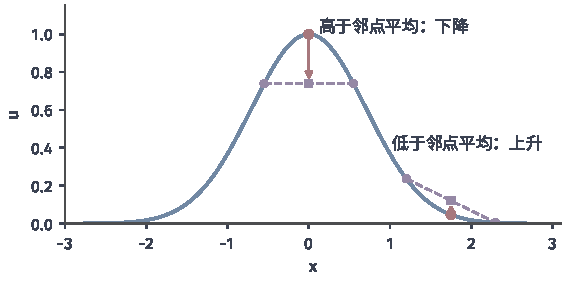
\includegraphics[width=96.0mm]{figures/06-differential-equations/02-partial-differential-equations/matplotlib/pdeprob-laplace-average/figure.pdf}
  \caption{二阶导数比较一点与其邻点的平均。蓝线为$u=\mathrm{e}^{-x^2}$，紫色虚线连接邻点$x_0\pm0.55$，紫色方块是两邻点的平均，红点是$u(x_0)$，红色箭头指示热方程下该点的变化方向。}
  \label{fig:pdeprob-laplace-average}
\end{BookInlineFigure}

在$d$维中，把两个邻点换成以$\bm{x}$为心、半径$r$的球面，同样的Taylor展开给出球面平均减去中心值约等于$\frac{r^{2}}{2d}\Delta u(\bm{x})$。这里用到单位球面上$n_in_j$的平均值，$i=j$时为$1/d$，$i\neq j$时为$0$。$f=0$时这个主项消失；事实上此时两者精确相等，这就是平衡状态下每一点的值等于周围平均的性质。

图~\ref{fig:pdeprob-three-evolutions}把同一个初始鼓包放进三个演化方程。热方程把它压低变宽，输运方程把它原样平移，波动方程把它分成两半向两侧传播。这三种行为分别对应抹平、搬运和分路传播，后面几章会分别加以证明。

\begin{BookInlineFigure}
  \centering
  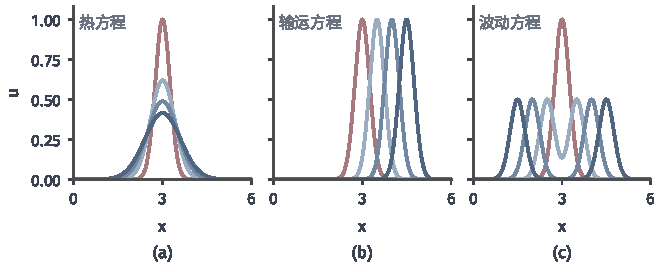
\includegraphics[width=112.0mm]{figures/06-differential-equations/02-partial-differential-equations/matplotlib/pdeprob-three-evolutions/figure.pdf}
  \caption{同一鼓包$u_0(x)=\exp(-(x-3)^2/(2\cdot0.25^2))$在实轴上的演化，红线为$t=0$，蓝色由浅到深为$t=0.5,1,1.5$。(a)$\partial_tu=0.1\,\partial_x^2u$，方差由$0.25^2$增至$0.25^2+0.2t$。(b)$\partial_tu+\partial_xu=0$，解为$u_0(x-t)$。(c)$\partial_t^2u=\partial_x^2u$，初速度为零，解为$\frac12[u_0(x-t)+u_0(x+t)]$。}
  \label{fig:pdeprob-three-evolutions}
\end{BookInlineFigure}

\paragraph{一般形式与线性程度}
上面的方程都是在每一点上把未知函数和它的有限个偏导数联系起来。把静态和演化两种情形放在一起，记自变量为$\bm{z}$：静态问题中$\bm{z}=\bm{x}$，演化问题中$\bm{z}=(\bm{x},t)$。用$D^{k}u$表示$u$的全部$k$阶偏导数。

\begin{definition}[偏微分方程]
\label{def:pdeprob-pde}
设$U$是自变量$\bm{z}$所在的开集，$u:U\to\mathbb{R}$是未知函数。若在$U$的每一点上，$u$及其不超过$m$阶的偏导数满足关系
\begin{equation}
  \mathcal{F}\bigl(\bm{z},u,Du,\ldots,D^{m}u\bigr)=0,
  \label{eq:pdeprob-general-form}
\end{equation}
且$\mathcal{F}$确实依赖某个$m$阶偏导数，则称它是$m$阶\term{偏微分方程}（partial differential equation, PDE）。
\end{definition}

方程按对最高阶导数和$u$的依赖方式分为几个层次，见表~\ref{tab:pdeprob-linearity}。线性方程的系数只依赖$\bm{z}$，算子$L$满足$L(au+bw)=aLu+bLw$；\term{半线性方程}（semilinear equation）的最高阶部分线性，且系数只依赖$\bm{z}$，低阶部分可以非线性；\term{拟线性方程}（quasilinear equation）的最高阶导数仍以一次形式出现，但系数可以依赖$u$和较低阶导数；\term{完全非线性方程}（fully nonlinear equation）对最高阶导数本身非线性。

\begin{BookInlineTable}
  \centering
  \begin{tabular}{lll}
    \toprule
    层次 & 例子 & 判断依据\\
    \midrule
    线性 & $\partial_tu-\nabla\cdot(\bm{A}(\bm{x})\nabla u)=f$ & 系数只依赖$\bm{x}$\\
    半线性 & $\partial_tu-\Delta u=u^{2}$ & 最高阶线性，低阶$u^{2}$\\
    拟线性 & $\partial_tu+u\,\partial_xu=0$ & $\partial_xu$的系数含$u$\\
    完全非线性 & $\partial_tu+\frac12(\partial_xu)^{2}=0$ & 最高阶导数出现平方\\
    \bottomrule
  \end{tabular}
  \caption{偏微分方程按线性程度的层次。}
  \label{tab:pdeprob-linearity}
\end{BookInlineTable}

这些区分影响求解方式。线性方程满足叠加：两个解的线性组合对相应右端仍是解，两个解之差满足右端为零的方程，这是证明唯一性时的基本手段。非线性方程没有这一性质，下面用拟线性方程$\partial_tu+u\,\partial_xu=0$算一个例子。

取两个解$u_1=1$和$u_2=x/(1+t)$。常数$u_1$的两个偏导数都是零，它满足方程。$u_2$的偏导数为
\[
  \partial_tu_2=-\frac{x}{(1+t)^{2}},\qquad
  u_2\,\partial_xu_2=\frac{x}{1+t}\cdot\frac{1}{1+t}=\frac{x}{(1+t)^{2}},
\]
两者相加为零。再看$w=u_1+u_2=1+x/(1+t)$，同样计算得
\[
  \partial_tw+w\,\partial_xw=-\frac{x}{(1+t)^{2}}+\Bigl(1+\frac{x}{1+t}\Bigr)\frac{1}{1+t}=\frac{1}{1+t}\neq0.
\]
两个解之和不是解。

其余几项的作用也可以逐一说清。阶数$m$决定经典意义下解要有几阶导数，也关系到要提供多少数据。系数是常数时，方程在平移下不变，可以用Fourier模式把求导变成乘法；系数随位置变化时这条路不再直接可用。源项$f$让方程非齐次，但在线性问题中可以通过取差消去。

\paragraph{向量未知量}
未知量也可以是向量场。把波动方程降阶就能得到一个例子，做法和常微分方程降阶相同。在一维中记$p=\partial_tu$，$q=\partial_xu$，波动方程$\partial_t^{2}u=c^{2}\partial_x^{2}u$和混合偏导相等分别给出
\[
  \partial_tp=c^{2}\partial_xq,\qquad \partial_tq=\partial_xp.
\]
记$\bm{w}=(p,q)^{\top}$，这是一个一阶方程组：
\begin{equation}
  \partial_t\bm{w}=\bm{B}\,\partial_x\bm{w},\qquad
  \bm{B}=\begin{pmatrix}0&c^{2}\\1&0\end{pmatrix}.
  \label{eq:pdeprob-first-order-system}
\end{equation}
$\bm{B}$的特征值是$\pm c$，恰好是波向两侧传播的速度。降阶用未知量的个数换取了导数的阶数；流体的速度场方程、电磁场方程也是这样的方程组。本部分以标量未知量为主。

\paragraph{函数作为无限维向量}
回到细棒，看空间离散后方程变成什么。在内部格点上用式~\eqref{eq:pdeprob-neighbor-average}近似$\partial_x^{2}u$，并取两端值为零，记$\bm{u}(t)=(u_1(t),\ldots,u_N(t))^{\top}$，热方程成为线性常微分方程组：
\begin{equation}
  \frac{\mathrm{d}\bm{u}}{\mathrm{d}t}=\bm{A}_h\bm{u},\qquad
  (\bm{A}_h\bm{u})_j=\frac{u_{j+1}-2u_j+u_{j-1}}{h^{2}}.
  \label{eq:pdeprob-semi-discrete}
\end{equation}
式中下标超出$1,\ldots,N$的格点值取为零，这样两端的零边值已经写进矩阵。

下面取$N=3$，$h=1/4$，逐项算出这个矩阵的特征值：
\[
  \bm{A}_h=16\begin{pmatrix}-2&1&0\\1&-2&1\\0&1&-2\end{pmatrix}.
\]
$\bm{A}_h$的第$k$个特征向量由$\sin(k\pi x_j)$组成，由和差化积，特征值是
\[
  \lambda_k=-\frac{4}{h^{2}}\sin^{2}\frac{k\pi h}{2},\qquad k=1,\ldots,N.
\]
代入$h=1/4$，得到
\[
  \lambda_1\approx-9.37,\quad \lambda_2=-32,\quad \lambda_3\approx-54.63.
\]

连续问题中对应的等式是
\[
  \partial_x^{2}\sin(k\pi x)=-k^{2}\pi^{2}\sin(k\pi x),
\]
前三个特征值约为$-9.87$、$-39.48$、$-88.83$。向量的分量对应函数在各点的值，矩阵$\bm{A}_h$对应算子$\partial_x^{2}$，特征向量对应正弦模式，矩阵的首末行编码了零边值。

这个类比在一个关键处失效。图~\ref{fig:pdeprob-spectrum-growth}显示，低频特征值随加密趋于$-k^{2}\pi^{2}$，但矩阵的谱范数约为$4/h^{2}$，$N\to\infty$时趋于无穷。

\begin{BookInlineFigure}
  \centering
  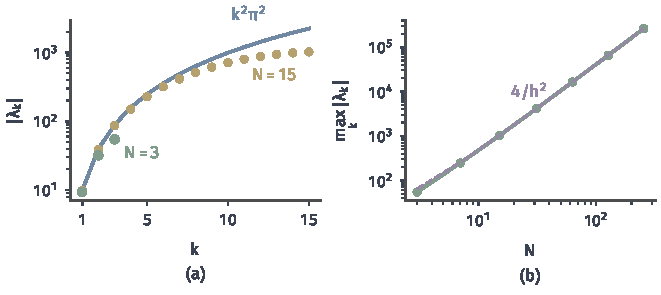
\includegraphics[width=112.0mm]{figures/06-differential-equations/02-partial-differential-equations/matplotlib/pdeprob-spectrum-growth/figure.pdf}
  \caption{式~\eqref{eq:pdeprob-semi-discrete}中矩阵的特征值。(a)第$k$个特征值的绝对值：$N=3$（绿）、$N=15$（黄）、连续问题的$k^2\pi^2$（蓝）。(b)最大特征值绝对值（绿）随$N$的增长，紫色虚线为$4/h^2$。}
  \label{fig:pdeprob-spectrum-growth}
\end{BookInlineFigure}

谱范数正是线性右端的Lipschitz常数。第~\ref{chap:ode-existence-continuation}章的存在性论证依赖右端的Lipschitz条件，而这里的常数随加密无界增长，极限算子$\partial_x^{2}$在$L^{2}(0,1)$或$C[0,1]$这样的空间上不是有界映射：它要消耗两阶导数。所以不能把偏微分方程直接当作无限维常微分方程来套用已有的定理。后面要靠别的结构，例如$\bm{A}_h$的特征值全部为负，来得到估计；这也是为什么必须先说清解和数据所在的空间。
